\usetikzlibrary{arrows, calc}
\begin{document}
\lecture{Implementierung von Datenbanksystemen}{IDB}
\title{Übungsblatt~12}
\subtitle{Planoperatoren, Nicht-algebraische Optimierung}
\maketitle

\begin{note}
	Achtung: Die Angabe von Aufgabe 3 enthält die Kostenformeln, die in Aufgabe 2 erarbeitet werden.
	Wir denken, dass das sowieso niemand bemerkt.
\end{note}

\section*{Lernziele}
\begin{itemize}
	\item Planoperatoralgorithmen
	\item Übersetzung von logischen Operatoren in Planoperatoren
	\item Kosten von Planoperatoren
	\item Kostenbasierte Anfrageoptimierung
	\item Optimierung in der Praxis
\end{itemize}

\section*{Literatur}
\GarciaMolinaFirst{15, 16}

\HaerderNintyNine{11, 12}

\ElmasriFive{16}

\section{Fragen zur Vorlesung}
\begin{enumerate}[a)]
\item Erläutern Sie den Ablauf eines Nested-Loop Joins.

\begin{solution}
Siehe VL-Folie~\NestedLoopJoin
\end{solution}

\cprotEnv
\begin{note}
\begin{lstlisting}
R,S: Relationen
for s in S:
  if(Vorbedingung auf S erfüllt):
    for r in R:
      if(Vorbedingung auf R erfüllt)
        if(Verbundbedingung erfüllt):
          Übernimm kombination in Ergebnis
\end{lstlisting}
Komplexität: $O(pages(R)\times pages(S))$
\end{note}

\item Erläutern Sie den Ablauf eines Hash Joins nach dem Classic-Hashing-Verfahren.

\begin{solution}
Siehe VL-Folie~\HashJoin
\end{solution}

\cprotEnv
\begin{note}
\begin{lstlisting}
R: Kleinere Relation
S: größere Reation
Fragmentiere R, sodass Fragmente R_i, i=1, ..., p 
	in Hauptspeicher passen
forall R_i:
  h: empty Hashtable
  forall r in R_i:// Befüllen
    insert r into h
  forall s in S: // Probing
    if(Verbundpartner in h):
      verbinde r mit s;
\end{lstlisting}
Komplexität: $O(p\times pages(S))$\\
Idealfall: p=1; R passt komplett in den Hauptspeicher.
\end{note}

\item Erläutern Sie den Unterschied zwischen logischen Operatoren und Planoperatoren.

	\begin{solution}
		Logische Operatoren repräsentieren die Semantik eines Operators.
		Sie sagen nichts darüber aus, wie der Operator implementiert ist, um diese Semantik zu erreichen.

		Ein Planoperator repräsentiert eine bestimmte Implementierung eines logischen Operators oder einer Gruppe von benachbarten logischen Operatoren.
	\end{solution}

\item Warum betrachtet man verschiedene Implementierungen von Operatoren?

	\begin{solution}
		Unterschiedliche Implementierungen können Vor- und Nachteile haben. Einfachstes Beispiel: Index-Scan ist jenseits der Grenztrefferrate sinnlos. Außerdem können die Implementierungen weiteren Einschränkungen unterliegen (Index vorhanden? Speicherplatzverbrauch bei Joins?). Je nach Einsatzzweck kann also eine andere Implementierung die beste sein.
	\end{solution}

\end{enumerate}
\begin{note}
Sollte das Übungsblatt zu lang sein, kann man je nach Verlauf der Übung
\begin{enumerate}
  \item eine der Wiederholungsfragen weglassen (sind sowieso 1:1 aus den Vorlesungsfolien übernommen)
  \item die kostenbasierte Optimierung abkürzen: Die Studenten erkennen bereits in Teilaufgabe 2a), dass ein Hash-Join schneller als ein Sort-Merge-Join und dieser wiederum schneller als ein Nested-Loop-Join ist. Deshalb kann man sich in Teilaufgabe b) immer darauf beschränken, nur die schnellste mögliche Join-Implementierung zu berechnen. Dadurch fallen auch fast alle Abschätzungen von Zwischenergebnisgrößen weg, was den zeitlichen Umfang deutlich begrenzt.
\end{enumerate}
\end{note}

\section{Kosten der Operatorausführung}
\label{sec:kosten}

\begin{enumerate}[a)]

\item Bei einer kostenbasierten Optimierung stellen die Kosten die Größe dar, die minimiert werden soll.
	Welche Werte könnte man bei der Optimierung von Datenbankanfragen in die Kosten einfließen lassen?

	\begin{solution}
		Z.\,B.\ Anzahl Blockzugriffe auf den Hintergrundspeicher, CPU-Zeit, Hauptspeicherbedarf, \ldots
	\end{solution}

\item \label{item:kostenformeln} Wir nehmen ein einfaches Kostenmodell an, das nur die Lese- und Schreibvorgänge auf dem Hintergrundspeicher berücksichtigt.
	Stellen Sie dafür Kostenformeln für die Planoperatoren Selektion, Projektion, Nested-Loop Join, Sort-Merge Join und Hash Join auf.
	Gehen Sie davon aus, dass die Eingaben vom Hintergrundspeicher gelesen werden müssen und die Ergebnisse direkt ausgegeben werden.
	\(B(S)\) gibt die Anzahl der Blöcke an, aus denen die Relation \(S\) besteht.

	\begin{solution}
		\begin{tabular}{l l p{5cm}}
			\hline
			\textbf{Implementierung} & \textbf{Kosten}          &                                                         \\ \hline
			Selektion(S)             & $B(S)$                   &                                                         \\ \hline
			Projektion(S)            & $B(S)$                   &                                                         \\ \hline
			NestedLoopJoin(S, T)     & $B(S) + B(S) \cdot B(T)$ &                                                         \\ \hline
			SortMergeJoin(S, T)      & $3 (B(S) + B(T))$        & Unter den in \SortMergeJoin genannten Voraussetzungen   \\ \hline
			HashJoin(S, T)           & $B(S) + B(T)$            & Classic Hashing, wenn eine Relation in den Puffer passt \\ \hline
		\end{tabular}

		Die Kosten werden einheitslos angegeben, da sie nur zum Vergleich zwischen den Operatoren dienen.

		In der Literatur finden sich je nach verwendetem Kostenmodell und berücksichtigten Kostentypen unterschiedliche Formeln. Eine gute Herleitung von Kostenformeln steht bei Garcia-Molina et al.
	\end{solution}

\item \label{item:pipelining} Pipelining bezeichnet das direkte Hintereinanderausführen mehrerer Operatoren, ohne die Zwischenergebnisse erst komplett zu erzeugen und auf den Hintergrundspeicher zu schreiben.
	Welche der aus der Vorlesung und Übung bekannten Planoperatoren eignen sich für Pipelining gut, welche nicht?

	\begin{solution}
		Als Quelle für Pipelining können alle Operatoren dienen.
		Zu beachten ist dabei aber, dass vom Quelloperator belegte Pufferkacheln nicht für den Zieloperator zur Verfügung stehen.
		Werden Table Scan und Index Scan als eigenständige Operatoren behandelt, wie wir das im Folgenden tun, dann werden sie immer per Pipelining mit dem folgenden Operator verbunden.
		Ein Table-Scan-Operator ohne Pipelining wäre sinnlos, da er lediglich die Relation umkopieren würde.

		Als Ziel für Pipelining sind alle Operatoren gut geeignet, die die Quelle nur einmal durchlaufen müssen, beispielsweise Selektion, Projektion oder auch die äußere Relation des Nested-Loop Joins.

		Der Nested-Loop Join ist gleichzeitig auch ein Beispiel für einen Operator, der sich nicht gut als Ziel für Pipelining eignet.
		Wird die innere Relation nicht zwischengespeichert, muss sie für jeden Durchlauf neu erzeugt werden.
	\end{solution}

\item Wie ändern sich die Kostenformeln aus Teilaufgabe \ref{item:kostenformeln}), wenn Pipelining eingesetzt wird?
Verwenden Sie \(C(S)\) für die Kosten zur Erzeugung der Zwischenergebnisrelation \(S\).

	\begin{solution}
		Dient ein Operator A als Eingabe für einen weiteren Operator B, können dessen Kosten in der Kostenformel für B an der Stelle der Blockzugriffe zum Lesen der Eingaberelation angesetzt werden.
		Blockzugriffe für das Schreiben des Ergebnisses werden nicht benötigt, da das Ergebnis direkt an den nächsten Operator oder an den Anwender weitergegeben wird.
		Die Gesamtkosten einer Anfrage sind dann einfach die Kosten der Wurzel im Operatorbaum.

		Beispiel: Selektion(S) hat mit Pipelining Kosten von C(S). Das bedeutet, dass die Kosten eines Selektionsoperators gerade so hoch sind wie die Erzeugungskosten seiner Eingabedaten. Das liegt daran, dass wir nur E/A-Kosten berücksichtigen und die Selektion selbst keine Ein- oder Ausgabe vornimmt.

		Als Kostenformeln mit Pipelining ergeben sich:

		\begin{tabular}{l l}
			\hline
			\textbf{Implementierung} 	& \textbf{Kosten}\\
			\hline
			Selektion(S)						& $C(S)$\\
			\hline
			Projektion(S)						& $C(S)$\\
			\hline
			TableScan	(S)							& $B(S)$\\
			\hline
			IndexScan(S)							& $a \cdot \left \lceil{ B(S) \cdot \mathrm{Selektivit"atsfaktor} }\right \rceil $\\
			\hline
			NestedLoopJoin(S, T)			& $C(S) + B(S) \cdot C(T)$\\
			\hline
			SortMergeJoin(S, T)				& $C(S) + C(T) + 2 (B(S) + B(T))$\\
			\hline
			HashJoin(S, T) 						& $C(S) + C(T)$\\
			\hline
		\end{tabular}

		Beim Index Scan wurden hier die Kosten eines wahlfreien Blockzugriffs als a-mal so hoch wie die eines sequentiellen Blockzugriffs angesetzt.
	\end{solution}

\end{enumerate}

\beamertxt{\pagebreak}

\section{Optimierung}

In dieser Aufgabe sollen verschiedene Implementierungsmöglichkeiten von Operatoren betrachtet und anhand ihrer Kosten verglichen werden.

\subsection*{Szenario}

Gegeben sind folgende Tabellen:

\texttt{L(\underline{l}, m[M], n[N]), m[M] NOT NULL, n[N] NOT NULL} \\
\texttt{M(\underline{m}, d, e)} \\
\texttt{N(\underline{n}, f, g)}

Folgende Attribute sind indiziert: \texttt{L.l, L.m, M.m, N.n}

Folgende Informationen sind jeweils im Systemkatalog abgelegt:

\begin{tabular}{p{2.5cm} p{10.97cm}}
	\hline
	\textbf{Bez\normaltxt[.]{eichnung}}  & \textbf{Beschreibung} \\
	\hline
	$B(S)$								& Anzahl der Blöcke, aus denen die Relation S besteht \\
	\hline
	$T(S)$								& Anzahl Tupel, die in der Relation S enthalten sind \\
	\hline
	$\mathrm{bfr}(S)$			& Mittlerer Blockungsfaktor der Relation S; ergibt sich aus $\frac{T(S)}{B(S)}$ \\
	\hline
	$V(S.a)$							& Anzahl der unterschiedlichen Werte, die für das Attribut a in S vorkommen \\
	\hline
\end{tabular}

\beamertxt{\pagebreak}

Folgende Werte sind bekannt:

$B(L) =       5.000 \\
B(M)  =       1.000 \\
B(N)  =         500 \\
T(L)  =     100.000 \\
T(M)  =      10.000 \\
T(N)  =       5.000 \\
V(N.f) =      3.000$

Vereinfachende Annahmen:
\begin{itemize}
	\item Wir betrachten nur die Kosten für Ein-/Ausgabe vom Hintergrundspeicher.
	\item Alle Indizes werden komplett im Arbeitsspeicher gehalten.
\end{itemize}

\beamertxt{\pagebreak}

\subsection*{Operatoren}

Die Kostenformeln sind aus Übungsblatt~12 bekannt:

Scan:\\
\begin{tabular}{p{3.2cm} p{5.5cm} p{4.5cm}}
  \hline
  \textbf{Impl\normaltxt[.]{ementierung}} &
  \textbf{Kosten} &
  \textbf{Einschränkungen} \\
  \hline
  TableScan (S) &
  $B(S)$ &
  \\
  \hline
  IndexScan(S) &
  $50 \cdot \left \lceil{ B(S) \cdot \mathrm{Selektivit"atsfaktor} }\right \rceil $ &
  Nur wenn geeigneter Index vorhanden (Kosten für wahlfreien Blockzugriff: 50) \\
  \hline
\end{tabular}

Join:\\
\begin{tabular}{p{3.7cm} p{4cm} p{5.5cm} }
	\hline
	\textbf{Impl\normaltxt[.]{ementierung}} 	& \textbf{Kosten}  &  \textbf{Einschränkungen}																								\\
	\hline
	NestedLoopJoin(S, T)			& $C(S) + B(S) \cdot C(T)$ 						& 																										\\
	\hline
	SortMergeJoin(S, T)				& $C(S) + C(T) + 2 \cdot (B(S) + B(T))$  	& Nur, wenn Gleichverbund  															\\
	\hline
	HashJoin(S, T) 					& $C(S) + C(T)$ 											& Nur, wenn Gleichverbund und eine Tabelle in den Puffer passt 	\\
	\hline
\end{tabular}

Weitere Operatoren:\\
\begin{tabular}{ p{3.7cm} p{4cm} p{5.5cm}}
	\hline
	\textbf{Operator} 	& \textbf{Kosten}  		&  \textbf{Bemerkungen}	\\
	\hline
	SEL(S)						& $C(S)$ 						& 										\\
	\hline
	PROJ(S)						& $C(S)$						& 										\\
	\hline
\end{tabular}

Dient die Ausgaberelation $S$ eines Operators A als Eingabe für einen weiteren Operator B, so sind die Kosten von A als $C(S)$ bereits in der Kostenformel für B enthalten.


\subsection*{Aufgaben}

\begin{enumerate}[a)]

	\item Gegeben seien Ausführungspläne für das folgende SQL-Statement.
	Bestimmen Sie jeweils die Ausführungskosten.

	\begin{lstlisting}
SELECT *
FROM   L JOIN M ON (L.m = M.m)
WHERE  L.l = 1000;
	\end{lstlisting}

	\begin{enumerate}[i)]

\item
Ausführungsplan 1:

	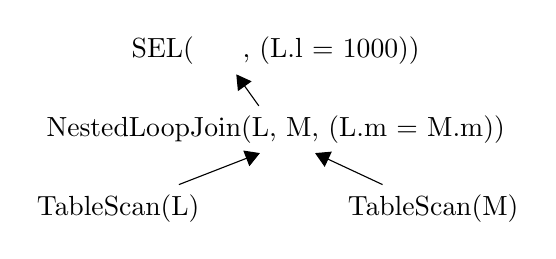
\begin{tikzpicture}
		\node (sel) at (0,0) {SEL( \hspace{0.5cm}, (L.l = 1000))};
		\node  (nested_loop) [below of = sel] {NestedLoopJoin(L, M, (L.m = M.m))};
		\node (L) [below of = nested_loop, xshift=-2cm] {TableScan(L)};
		\node (M) [below of = nested_loop, xshift=2cm] {TableScan(M)};
		\draw[-triangle 60] (L) -- ($(nested_loop.south) + (-0.2,0)$);
		\draw[-triangle 60] (M) -- ($(nested_loop.south) + (0.5,0)$);
		\draw[-triangle 60] (nested_loop) -- ($(sel.south) + (-0.5,0)$);
	\end{tikzpicture}

\begin{solution}
Der Nested-Loop-Join ist, bei den in dieser Aufgabe angesetzten Kostenformeln, der einzige nicht symmetrische Operator, d.\,h.\ für den Nested-Loop-Join ergeben sich unterschiedliche Kosten für Nested-Loop-Join(A, B) und Nested-Loop-Join(B, A).
Exemplarisch wird in dieser Aufgabe die Berechnung beider Varianten gezeigt, im Folgenden jedoch nur noch die kostengünstigere Variante betrachtet.

	\textbf{Ausführungsplan 1:}
	\begin{align*}
		\mathtt{TableScan}(L)         & = B(L) = 5.000                                                         \\
		\mathtt{TableScan}(M)         & = B(M) = 1.000                                                         \\
		\mathtt{NestedLoopJoin}(L, M) & = C(L) + B(L) \cdot C(M) =                                             \\
		                              & =\mathtt{TableScan}(L)+ B(L) \cdot \mathtt{TableScan}(M) =  5.005.000  \\
		\mathtt{NestedLoopJoin}(M, L) & = C(M) + B(M) \cdot C(L) =                                             \\
		                              & = \mathtt{TableScan}(M) + B(M) \cdot \mathtt{TableScan}(L) = 5.001.000
	\end{align*}
	$\Rightarrow$ Kosten: $5.001.000$ \\
	\end{solution}

	\begin{note}
	Für die Selektion fallen keine weiteren Kosten mehr an -- siehe Aufgabenstellung.
	\end{note}

\item
Ausführungsplan 2:

	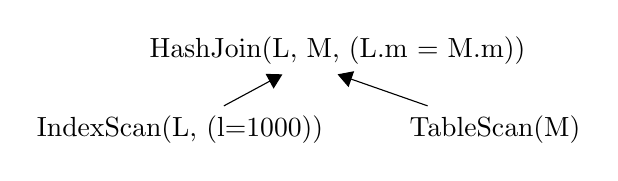
\begin{tikzpicture}
		\node (join) at (0,0) {HashJoin(L, M, (L.m = M.m))};
		\node (L) [below of = join, xshift=-2cm] {IndexScan(L, (l=1000))};
		\node (M) [below of = join, xshift=2cm] {TableScan(M)};
		\draw[-triangle 60] (L) -- ($(join.south) + (-0.7,0)$);
		\draw[-triangle 60] (M) -- (join.south);
	\end{tikzpicture}

	\begin{solution}
	\textbf{Ausführungsplan 2:}
	\begin{align*}
		\mathtt{IndexScan}(L)  & = 50                                                                 \\
		                       & \text{L.l ist PK, daher liefert er nur ein Tupel und der}           \\
		                       & \text{Selektivitätsfaktor ist $\frac{1}{T(L)} = \frac{1}{100000}$} \\
		\mathtt{TableScan}(M)  & = 1.000                                                              \\
		\mathtt{HashJoin}(L,M) & = C(L) + C(M) = \mathtt{IndesScan}(L) + \mathtt{TableScan}(M) =      \\
		                       & =  50 + 1000
	\end{align*}
	$\Rightarrow$ Kosten: $1.050$

	Auch für ein Tupel muss man einen ganzen Block lesen.
	Für das wahlfreie Lesen eines Blocks fallen nach den gegebenen Formeln Kosten von 50 an.

	\textbf{Erkenntnis:} Kleine Änderungen können unglaubliche Ergebnisse erzielen.
	\end{solution}

\item
Ausführungsplan 3:\deepen

\cprotEnv
\begin{normalText}
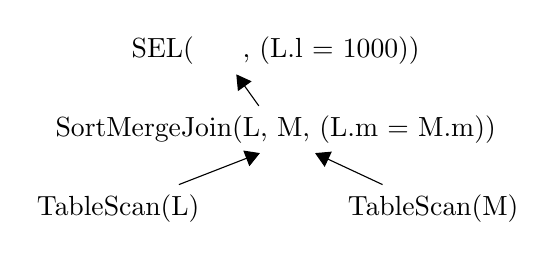
\begin{tikzpicture}
		\node (sel) at (0,0) {SEL( \hspace{0.5cm}, (L.l = 1000))};
		\node  (sort_merge) [below of = sel] {SortMergeJoin(L, M, (L.m = M.m))};
		\node (L) [below of = sort_merge, xshift=-2cm] {TableScan(L)};
		\node (M) [below of = sort_merge, xshift=2cm] {TableScan(M)};
		\draw[-triangle 60] (L) -- ($(sort_merge.south) + (-0.2,0)$);
		\draw[-triangle 60] (M) -- ($(sort_merge.south) + (0.5,0)$);
		\draw[-triangle 60] (sort_merge) -- ($(sel.south) + (-0.5,0)$);
	\end{tikzpicture}
\end{normalText}

\begin{note}
\textbf{Ausführungsplan 3:}

	$\mathtt{SortMergeJoin}(L,M) = C(L) + C(M) + 2(B(L) + B(M))$ \\
	$C(L) = \mathtt{TableScan}(L) = 5.000$  \\
	$C(M) = \mathtt{TableScan}(M) = 1.000$ \\
	$\Rightarrow$ Kosten: $18.000$
\end{note}

\item
Ausführungsplan 4:\deepen

\cprotEnv
\begin{normalText}
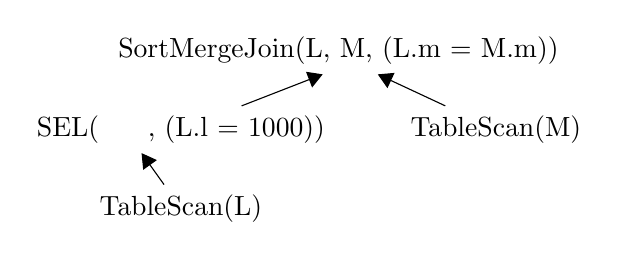
\begin{tikzpicture}
		\node  (sort_merge)  at (0,0) {SortMergeJoin(L, M, (L.m = M.m))};
		\node (sel) [below of=sort_merge, xshift=-2cm] {SEL( \hspace{0.5cm}, (L.l = 1000))};
		\node (L) [below of = sel] {TableScan(L)};
		\node (M) [below of = sort_merge, xshift=2cm] {TableScan(M)};
		\draw[-triangle 60] (sel) -- ($(sort_merge.south) + (-0.2,0)$);
		\draw[-triangle 60] (M) -- ($(sort_merge.south) + (0.5,0)$);
		\draw[-triangle 60] (L) -- ($(sel.south) + (-0.5,0)$);
	\end{tikzpicture}
\end{normalText}

\begin{note}
\textbf{Ausführungsplan 4:}

	$\mathtt{SortMergeJoin}(L,M) = C(L) + C(M) + 2(B(L) + B(M))$ \\
	$C(L) = \mathtt{TableScan}(L) = 5.000$  \\
	$C(M) = \mathtt{TableScan}(M) = 1.000$ \\
	$B(M) = 1.000$\\
	$B(L) = 1$\\
	$\Rightarrow$ Kosten: $8.002$
\end{note}

\end{enumerate}
\beamertxt{\pagebreak}

	\item Wählen Sie für die folgenden logischen Ausführungspläne passende Planoperatoren und Ausführungsreihenfolgen aus.
Gehen Sie davon aus, dass 700 Kacheln Hauptspeicher zur Verfügung stehen.
Eine Kachel sei dabei gerade so groß wie eine Seite.

Um die Zahl der möglichen Varianten in Grenzen zu halten, können Sie für die Relationen, die in die JOINS einfließen, auf die Berücksichtigung von Index-Scans verzichten und nur Table-Scans einsetzen.

	\begin{enumerate}[i)]

		\item \label{Optimierung2_1} Gegeben sind das folgende SQL-Statement und der zugehörige logische Aus"-füh"-rungs"-plan.

		\begin{minipage}{5.5cm}
		\begin{lstlisting}
SELECT *
FROM   L, M, N
WHERE  L.m = M.m
       AND L.n = N.n;
		\end{lstlisting}
		\end{minipage}
		\begin{minipage}{7cm}
		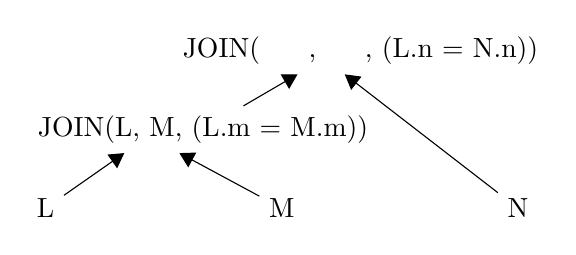
\begin{tikzpicture}
			\node (join1) at (0,0) {JOIN( \hspace{0.5cm}, \hspace{0.5cm}, (L.n = N.n))};
			\node (join2) [below of =join1, xshift=-2cm] {JOIN(L, M, (L.m = M.m))};
			\node (L) [below of = join2, xshift=-2cm] {L};
			\node (M) [below of =join2, xshift=1cm] {M};
			\node (N) [below of = join2, xshift=4cm] {N};
			\draw[-triangle 60] (join2) -- ($(join1.south) + (-0.8,0)$);
			\draw[-triangle 60] (L) -- ($(join2.south) + (-1,0)$);
			\draw[-triangle 60] (M) -- ($(join2.south) + (-0.3,0)$);
			\draw[-triangle 60] (N) -- ($(join1.south) + (-0.2,0)$);
		\end{tikzpicture}
		\end{minipage}

\begin{solution}
		Ohne Verwendung von Index-Scans sind unsere Optionen die drei verschiedenen Join-Implementierungen und die beiden möglichen Reihenfolgen der Joins.
		Das gibt schon $3 \cdot 2 = 6$ Möglichkeiten.
		Dazu kann man sparen, wenn man Zwischenergebnisse speichert.
		(Zuerst M mit N zu joinen funktioniert nicht, da sie keine gemeinsamen Attribute haben.
		Auch ein Kreuzprodukt von M und N ergibt aufgrund der Größe und den Erzeugungskosten des Zwischenergebnisses keinen Sinn.)
		\nt{$10K \cdot 5K = 50Mio$ Tupel, benötigen ca 10Mio Blöcke, Kosten vgl. NLJoin $5k \cdot 10k + 5k \approx 50M$}

		\paragraph{\color{solutioncolor}Reihenfolge: \texttt{JOIN(JOIN(L, M), N)}}

		\begin{enumerate}[1.]

			\item \texttt{JOIN(L, M)}
			  \begin{itemize}
				  \item Gleichverbund erlaubt SortMergeJoin.
				  \item HashJoin ist nicht möglich, da keine Relation in den Speicher passt.
			  \end{itemize}
			  \texttt{NestedLoopJoin(M, L):} $1.000 + (1.000 \cdot 5.000) = 5.001.000$ \\
			  \texttt{SortMergeJoin(L, M):} $5.000 + 1.000 + 2 \cdot (5.000 + 1.000) = \underline{18.000}$ \\

			  \textbf{Abschätzung der Zwischenergebnisgrößen -- Variante 1:}

			  \texttt{L.m} und \texttt{L.n} sind Fremdschlüssel, \texttt{M.m} und \texttt{N.n} Primärschlüssel und damit \texttt{UNIQUE}.
			  Damit hat jedes Tupel in \texttt{L} beim Gleichverbund höchstens einen Partner.
			  Da \texttt{L.m} und \texttt{L.n} außerdem \texttt{NOT NULL} sind, hat jedes Tupel in \texttt{L} beim Gleichverbund genau einen Partner.
			  Die Anzahl der Ergebnistupel ist damit $T(L)=100.000$.

			  Die Größe eines Tupels ist die Summe der Einzelgrößen: \\
			  $\mathrm{bfr}(L) = 20$, $\mathrm{bfr}(M)= \mathrm{bfr}(N) = 10$

			  $\Rightarrow \mathrm{bfr}(\texttt{JOIN(L, M)}) = \mathrm{bfr}(\texttt{JOIN(L, N)})= \frac{1}{0.05 + 0.1} = \lfloor6,67\rfloor = 6$ (der Rest ist Verschnitt).
			  Das bedeutet $100.000$ Tupel benötigen $16.667$ Blöcke!

			  Diese Abschätzung geht davon aus, dass alle Blöcke bis auf den Verschnitt komplett mit Tupeln gefüllt sind.
			  Bei variabel langen Sätzen wird die Satzlänge als statistisch unabhängig vom Join-Prädikat angenommen, so dass der durchschnittliche Blockungsfaktor auch für die am Join beteiligten Sätze repräsentativ ist.
			  Außerdem wird der Effekt vernachlässigt, dass nach dem Join weniger Verschnitt auftreten kann als vorher.

			  \textbf{Abschätzung der Zwischenergebnisgrößen -- Variante 2:}

			  Bei \texttt{JOIN(L, M)} hat jedes Tupel aus \texttt{M} im Mittel 10 Partner.
			  \texttt{B(JOIN(L, M))} ist daher $5000+10 \cdot 1000 = 15.000$ (jedes Tupel aus \texttt{L} kommt 1x, jedes aus \texttt{M} 10x vor).

			  Bei \texttt{JOIN(L, N)} hat jedes Tupel aus \texttt{N} im Mittel 20 Partner.
			  \texttt{B(JOIN(L,N))} ist daher $5000+20 \cdot 500 = 15.000$.

			  Wir verwenden die Werte aus Variante 1.
			  Variante 2 wäre aber genauso zulässig.

			\item \texttt{JOIN(JOIN(L, M), N)}
			  \begin{itemize}
				  \item Wir verwenden das günstigste Zwischenergebnis aus dem ersten JOIN.
				  \item Relation \texttt{N} passt in den Speicher, deshalb ist ein HashJoin möglich.
			  \end{itemize}

			  \texttt{NestedLoopJoin((L, M), N):} $18.000 + 16667 \cdot 500 = 8.351.500$ \\
			  \texttt{SortMergeJoin((L, M), N):} $18.000 + 500 + 2 \cdot (16.667 + 500) = 52.834$ \\
			  \texttt{HashJoin((L, M), N):} $18.000 + 500 = \underline{18.500}$ \\

		\end{enumerate}

		Hier kann man sich natürlich die Frage stellen, ob die beiden Joins für das Pipelining gleichzeitig in den Hauptspeicher passen, genauer, ob der letzte Schritt des Sort-Merge-Joins Zeitgleich zum Hash-Join ausgeführt werden kann.
		Dem Sort-Merge-Join steht zu Beginn der gesamte Arbeitsspeicher zur Verfügung, weswegen er die Relation L in $\lceil 1000/700\rceil = 2$, die Relation M in $\lceil 5000 / 700 \rceil = 8$ Teillisten auf, welche einzeln sortiert auf dem Laufwerk gespeichert werden.
		Im letzten Schritt wird nun von jeder dieser Teillisten ein Block geladen, das passende Tupel generiert und an den Hash-Join weitergeleitet.
		Damit werden 10 (+1 für das Tupel selber) Kacheln benötigt.
		Relation L benötigt 500 Kacheln im Hauptspeicher für die Hash-Tabelle, es stehen $700-11=689$ zur Verfügung.
		Das reicht aus.

		\paragraph{\color{solutioncolor}Reihenfolge: \texttt{JOIN(JOIN(L, N), M)}}

		\begin{enumerate}[1.]

			\item \texttt{JOIN(L, N)}

			  \texttt{NestedLoop(N, L):} $500 + (500 \cdot 5.000) = 2.500.500$ \\
			  \texttt{SortMerge(L, N):} $5.000 + 500 + 2 \cdot (5.000 + 500) = 16.500$ \\
			  \texttt{HashJoin(L, N):} $5.000 + 500 = \underline{5.500}$ \\

			\item \texttt{JOIN(JOIN(L, N), M)}

			  \texttt{NestedLoop(M, (L, N)):} $1.000 + (1.000 \cdot 5.500) = 5.501.000$ \\
			  \texttt{SortMerge((L, N), M):}  $5.500 + 1.000 + 2 \cdot (16.667 + 1.000) = \underline{41.834}$ \\
			\texttt{HashJoin((L, N), M):} Nicht möglich, da Zwischenergebnis zu groß.

		\end{enumerate}

\end{solution}

		\item Gegeben sind das folgende SQL-Statement und der zugehörige logische Aus"-füh"-rungs"-plan.

		\begin{minipage}{5.5cm}
		\begin{lstlisting}
SELECT *
FROM   L, M, N
WHERE  L.m > M.m
       AND L.n = N.n;
		\end{lstlisting}
		\end{minipage}
		\begin{minipage}{7cm}
		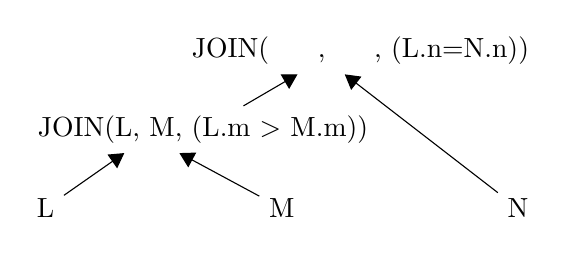
\begin{tikzpicture}
			\node (join1) at (0,0) {JOIN( \hspace{0.5cm}, \hspace{0.5cm}, (L.n=N.n))};
			\node (join2) [below of =join1, xshift=-2cm] {JOIN(L, M, (L.m $>$ M.m))};
			\node (L) [below of = join2, xshift=-2cm] {L};
			\node (M) [below of =join2, xshift=1cm] {M};
			\node (N) [below of = join2, xshift=4cm] {N};
			\draw[-triangle 60] (join2) -- ($(join1.south) + (-0.8,0)$);
			\draw[-triangle 60] (L) -- ($(join2.south) + (-1,0)$);
			\draw[-triangle 60] (M) -- ($(join2.south) + (-0.3,0)$);
			\draw[-triangle 60] (N) -- ($(join1.south) + (-0.2,0)$);
		\end{tikzpicture}
		\end{minipage}

		\begin{solution}
		Unsere Optionen bleiben im Prinzip gleich.
		Allerdings beherrscht nur der Nested-Loop-Join etwas anderes als den Gleichverbund.

		\paragraph{\color{solutioncolor}Reihenfolge: \texttt{JOIN(JOIN(L, M), N)}}

		\begin{enumerate}[1.]

			\item \texttt{JOIN(L, M)}

			  \texttt{NestedLoopJoin(M, L):} $1.000 + (1.000 \cdot 5.000) = \underline{5.001.000}$

			  \textbf{Abschätzung der Zwischenergebnisgrößen:}

			  Bei \texttt{JOIN(L, M)} wird jedes Tupel aus L mit im Mittel $\frac{T(M)}{2} =5.000$ Tupeln aus M gejoint (oder umgekehrt).\\
			  Die Anzahl der Tupel ist daher $\frac{T(L) \cdot T(M)}{2}=500.000.000$.\\
			  Die Größe eines Tupels ist die Summe der Einzelgrößen:\\
			  $bfr(L) = 20\Rightarrow \frac{1}{20}$~[Blöcke], $bfr(M) = 10\Rightarrow \frac{1}{10}$ [Blöcke].\\
			  Tupelgröße: $\frac{1}{10}+\frac{1}{20} = \frac{3}{20}$ [Blöcke].\\
			  $\Rightarrow bfr(\texttt{JOIN(L, M)}) = \left\lfloor\frac{1}{\frac{3}{20}}\right\rfloor = \left\lfloor \frac{20}{3}\right\rfloor =  \lfloor6,67\rfloor = 6$.
			  Damit hat das Zwischenergebnis von \texttt{B(JOIN(L, M))} 83.333.334 Blöcke.

			  Der Abschätzung liegen die gleichen Annahmen zugrunde wie Variante 1 in Teilaufgabe \ref{Optimierung2_1}).

			  Für \texttt{JOIN(L, N)} gilt das oben in Teilaufgabe \ref{Optimierung2_1}) ermittelte Ergebnis (16.667 Blöcke).

			\item \texttt{JOIN(JOIN(M, L), N)}

			  \texttt{NestedLoopJoin((M, L), N):} $5.001.000 + (83.333.334 \cdot 500) \approx 42$ Milliarden
			  \texttt{NestedLoopJoin(N, (M, L)):} $500 + (500 \cdot 5.001.000) = 2.500.500.500 42 \approx 2,5$ Milliarden

			\begin{note}
			(Table-Scan)

			\texttt{NestedLoopJoin((M, L), N):} $5.001.000 + (83.333.334 \cdot 50 \cdot \left \lceil{ 500 \cdot \frac{1}{5000} }\right \rceil ) \approx 4$ Milliarden (Index-Scan mit Selektivitätsfaktor $\frac{1}{T(N)}$, da Gleichverbund mit Primärschlüssel)

			Index-Scan hier nur beispielhaft als Anmerkung, da er sonst bei allen anderen Varianten auch berücksichtigt werden müsste und das die Aufgabe noch mal deutlich verlängern würde.
			\end{note}

			  \texttt{SortMergeJoin((M, L), N):} $5.001.000 + 500 + 2 \cdot (83.333.334 + 500) = 171.669.168$ \\
			  \texttt{HashJoin((M, L), N):} $5.001.000 + 500 = \underline{5.001.500}$

		\end{enumerate}

		\paragraph{\color{solutioncolor}Reihenfolge: \texttt{JOIN(JOIN(L, N), M)}}

		\begin{enumerate}[1.]

			\item \texttt{JOIN(L, N)} (wie in Teil \ref{Optimierung2_1})

			  \texttt{NestedLoopJoin(N, L):} $500 + (500 \cdot 5.000) = 2.500.500$ \\
			  \texttt{SortMergeJoin(L, N):} $5.000 +500 + 2 \cdot (5.000 + 500) = 16.500$ \\
			  \texttt{HashJoin(L, N):} $5.000 + 500 = \underline{5.500}$ \\

			\item \texttt{JOIN(JOIN(L, N), M)}

			  \texttt{NestedLoopJoin(M, (L, N)):} $1.000 + (1.000 \cdot 5.500) = \underline{5.501.000}$

		\end{enumerate}

		\textbf{Erkenntnis:} Mit den vorgegebenen Operatoren hat das Selektionsprädikat große Auswirkungen auf die Ausführungskosten.
		Beste Lösung ist 5.001.500 gegenüber 18.500 oben.
		Dabei ist der einzige Unterschied, dass im SQL-Statement "`$>$"' statt "`$=$"' steht.

		\end{solution}

	\end{enumerate}

\end{enumerate}

\section{Optimierung im Betrieb -- Beispiele}

Große Datenbanksysteme wie beispielsweise Oracle bieten Administratoren die Möglichkeit,
im Betrieb Einfluss auf bestimmte Optimierungsparameter zu nehmen.
Welche Informationen benötigt der Administrator und wie könnten Schnittstellen für diese Einflussnahme aussehen?

\begin{note}
Diskussionsaufgabe! Im folgenden ist beispielhaft beschrieben,
welche Möglichkeiten Oracle unter anderem bietet.

Darüber hinaus sind viele weitere denkbar und auch implementiert.
\end{note}

\cprotEnv
\begin{solution}
Wie Sie in den letzten Blättern kennengelernt haben,
nutzen Datenbanksysteme häufig bereits verschiedenste Algorithmen,
um das Leistungsverhalten zu steigern.
Dazu müssen verschiedene Hilfsstrukturen mitgeführt werden.

Der Administrator als Mensch hat unter Umständen durch Kenntnis
des gesamten Systems (also Hardware, Betriebssystem, Anwendung etc.)
die Möglichkeit, bessere Aussagen zu möglichen Optimierungen zu treffen,
als es das Datenbankverwaltungssystem durch reines Mitführen von Statistiken kann.

Damit der Administrator die vom System getroffenen Entscheidungen
jedoch bewerten kann, benötigt er Zugriff auf die internen Statistiken,
auf Basis derer das Datenbankverwaltungssystem die Entscheidungen trifft.

    Bei Oracle ist es nicht nur möglich,
    die internen Statistiken über die Datenbank selbst zu betrachten.
    Es werden darüber hinaus auch Statistiken
    über die ausgeführten SQL-Anfragen gesammelt,
    wie z.\,B. Ausführungszeiten, generierte Ausführungspläne
    etc.\footnote{\url{http://docs.oracle.com/cd/B19306_01/server.102/b14211/sql_1016.htm\#i26072}}

    Stellt der Administrator nun fest, dass für eine bestimmte Anfrage
    regelmäßig ein (in der Praxis) schlechter Ausführungsplan gewählt wird,
    kann er z.B. mit sogenannten \emph{HINTS} die Ausführung beeinflussen.
    Dabei wird in die SQL-Anfrage selbst ein Kommentar geschrieben,
    der vom Optimierer interpretiert
    wird.\footnote{\url{http://docs.oracle.com/cd/B19306_01/server.102/b14211/hintsref.htm}}

    Ein solcher HINT könnte z.\,B. so aussehen:

\begin{lstlisting}
    SELECT /*+ USE_NL(e d) */ e.fname, e.lname, e.addr
        FROM employee e
        JOIN department d
        ON d.num = e.dep
        WHERE d.name = 'Research';
\end{lstlisting}

    Damit wird dem Optimierer empfohlen, einen Nested-Loop-Join zu verwenden.
    Zu beachten ist jedoch, dass es sich dabei
    -- wie der Begriff \emph{HINT} schon andeutet --
    nicht um eine Anweisung handelt,
    sondern wie gesagt vielmehr um eine \textbf{Empfehlung}.
    Der Optimierer kann sich trotzdem darüber hinwegsetzen.
    Der Administrator erkennt dies dann wieder in den Statistiken.


    Das ständige (oder regelmäßige) Mitführen von Statistiken generiert
    auf dem System allerdings zusätzliche Last,
    entweder durch ständiges Aktualisieren von Statistikdaten
    oder durch regelmäßige Aktualisierungsläufe.

    Oracle bietet daher einen weiteren ganz grundsätzlichen Ansatz an.
    Es ist möglich, den kostenbasierten Optimierer zu deaktivieren
    und Ausführungspläne z.\,B. nach festen Regeln erstellen zu
    lassen.\footnote{\url{http://docs.oracle.com/cd/B19306_01/server.102/b14211/optimops.htm}}
    Das bietet den Vorteil, dass auf das Mitführen von Statistiken
    (vor allem wie viele Tupel in einer Relation sind, Selektivitäten etc.)
    weitgehend verzichtet werden kann.
    Ist also absehbar,
    dass der mit den Statistiken verbundene Aufwand größer ist
    als der Nutzen der kostenbasierten Wahl der Ausführungspläne,
    kann auch
    auf den kostenbasierten Optimierer komplett verzichtet werden.

    Weitere mögliche Ideen, unabhängig vom verwendeten System:
    \begin{itemize}
        \item Wenn häufig eine komplizierte JOIN-Abfrage durchgeführt wird:
            \textbf{Materialisierte Sicht} anlegen
            (und die Anfragen daran anpassen oder dem Optimierer beibringen,
            dass er die Sicht automatisch nutzen kann)
        \item Wenn in der Selektion häufig ein Ausdruck verwendet wird,
            der die Nutzung eines bisher verfügbaren Index unmöglich macht:
            \textbf{Function-Based Index} über diesen Ausdruck anlegen
        \item Puffer vergrößern
        \item schnellere / besser geeignete Hintergrundspeicher
    \end{itemize}
\end{solution}


\begin{deeper}
\section{Programmieraufgabe 8: Metadatenbank}

\subsection{Aufgabenstellung}
\begin{enumerate}
	\item Implementieren Sie eine Klasse, die die Schnittstelle \beamertxt{\linebreak}\texttt{idb.meta.Metadata} implementiert.
		Beachten Sie die Dokumentation der Methoden in der Schnittstelle.
	\item Tragen Sie den Konstruktor Ihrer Klasse in \texttt{idb.construct.Util} in der Methoden \texttt{createMetadata()} ein.
		Diese Methode erhält neben dem \texttt{DBBuffer} einen \texttt{idb.meta.FileCache} und einem Array mit 6 Strings, die als Pfade für beliebige Dateien verwendet werden können.
		Diese Dateien werden beim Aufruf bereits erzeugt und leer sein.
	\item Tragen Sie außerdem einen Konstruktor Ihrer Klasse in \texttt{idb.construct.Util} in der Methode \texttt{reloadMetadata()} ein.
		Diese Methode erhält die selben Parameter wie \texttt{createMetadata}, soll jedoch keine neue Datenbank anlegen, sondern diese wiederherstellen
	\item Sorgen Sie dafür, dass Sie alle Tests aus der Klasse \texttt{MetaTests} erfüllen.
	Sie können diese Testfälle mit \lstinline|ant Meilenstein8a| ausführen.
	\item Sorgen Sie dafür, dass Sie alle Tests aus der Klasse \texttt{LoadedMetaTests} erfüllen.
	Sie können diese Testfälle mit \lstinline|ant Meilenstein8b| ausführen.
	\item Die Abgabe auf GitLab erfolgt zeitgleich mit der Abgabe der Zusatzaufgaben des nächsten Übungsblattes auf StudOn. Markieren Sie hierfür Ihre Abgabe mit dem Tag "`Aufgabe-8"'.
\end{enumerate}

\subsection{Hinweise}
\begin{itemize}
	\item Der \texttt{FileCache} bietet angenehme Methoden zur Produktion von TIDFiles und KeyRecordFiles aus Pfaden.
		Verwenden Sie diese anstelle der in \texttt{idb.construct.Util} von Ihnen eingetragenen Methoden um Probleme mit mehreren (verschiedenen) Instanzen von KeyRecord / TIDFile auf geteilten Dateien zu verhindern.
		Rufen Sie niemals \texttt{close} auf den Dateien aus dem FileCache auf, da dieses für Sie übernommen wird.
	\item Der \texttt{FileCache} ist nicht zur Erzeugung neuer Dateien geeignet. Rufen Sie dafür weiterhin die von Ihnen in \texttt{idb.construct.Util} eingetragenen Funktionen auf.
		Beachten Sie, dass Sie für die selbst generierten und nicht aus FileCache stammenden Blockfiles und KeyRecordFiles selbstständig \texttt{close} aufrufen müssen.
		Um diese Unterscheidung nicht dauerhaft vornehmen zu müssen, hilft es, die erzeugten Dateien schnell zu schließen und dann über den \texttt{FileCache} erneut öffnen zu lassen.
	\item Beachten Sie, dass ein Puffer wie im Clock-Puffer Referenzen auf bereits mit \texttt{unfix} freigegebene Kacheln beibehält, bis die jeweilige Kachel wieder gebraucht wird.
		Wenn Sie nun \texttt{close} auf den Blockfiles aufrufen, geraten Sie bei späteren \texttt{fix} Aufrufen dann in problematische Fehler oder Randfälle.
		Bei einer korrekten Implementierung des Clock-Puffers inklusive des Zurücksetzens von \texttt{setDirty} im \texttt{flush} können Sie mit eben diesem \texttt{flush} dieses Problem umgehen.
		Notfalls können Sie auch testweise im Testfall den Clock-Puffer durch den sehr viel langsameren Simple-Buffer ersetzen, indem Sie die entsprechenden Zeilen im Setup ein- und auskommentieren.
	\item Unsere Indexstrukturen sind ausschließlich als Sekundärstrukturen verwendbar. Aufgrund der Einschränkungen der Hash-Implementierung können diese nicht als Primärstrukturen verwendet werden.
	\item Um unsere in der letzten Aufgabe erstellte Funktion zum Löschen von Tupeln einer Relation zu verwenden, verlangen wir für jede Relation einen Sekundärindex, aufgebaut auf dem Primärschlüssel.
	\item Während es Ihnen freigestellt ist, wie Sie Ihre sechs Dateien verwenden, empfehlen wir zwei Tabellen mit jeweils einer TIDFile und einem Index auf dem Primärschlüssel als KeyRecordFile / LinHash.
	\item Wir empfehlen die folgenden zwei Tabellen: 
\begin{enumerate}
\item Attributes(\textit{Name}: String, \textit{Rel}: String, \textit{Type}: String, \textit{Pos}: Int, \textit{PrimaryKey}: Boolean, \textit{SurrogateKey}: Boolean, \textit{\_Surrogate}: Int): Bei \textit{\_Surrogate} handelt es sich um den Surrogat-Primärschlüssel
\item Files(\textit{Path}: String, \textit{Relation}: String, \textit{Type}: String, \textit{BlockSize}: Int):
\textit{Path} bezeichnet den Primärschlüssel, der \textit{Type}-String kodiert ob es sich um eine \textit{TID-File}, den \textit{Regulärbereich} eines Hashing oder um den \textit{Overflowbereich} des Hashing handelt.
Im Falle einer \textit{Indexdatei} (Hashing, Regulär und Overflow) muss zusätzlich im \textit{Type}-String kodiert werden, welches Attribut in diesem Index als Schlüssel verwendet wird, üblicherweise durch seine (eindeutige) Position in der Relation.
\end{enumerate}
Die Verwendung von zwei Tabellen dieser festen Struktur hat den Vorteil, die Planoperatoren der letzten Aufgabe in der Meta-Datenbank verwenden zu können.
		Im Gegensatz zur echten Datenbank sind hier die Attributnamen und -typen jedoch unveränderlich, sodass die entsprechenden \texttt{NamedCombinedRecord} zur Pogrammierzeit bestimmt werden können.
		Dabei sind die Attribute wie folgt zu verstehen:
		\begin{enumerate}
			\item \textit{Attributes.Name}: Der (in einer Relation eindeutige) Name eines Attributes. Attributnamen bestehen ausschließlich aus den Buchstaben A-Z und a-z.
			\item Attributes.Rel: Der Name der Relation, in dem dieses Attribut definiert sein soll.
			\item \textit{Attributes.Type}: Der Typ des Attributes. In unserer Datenbank entweder \texttt{DBString}, \texttt{Bool} oder \texttt{IntegerKey}. Die Darstellung als String empfiehlt sich einfach zu halten (z.B. durch einen Buchstaben).
			\item \textit{Attributes.Pos}: Die Position dieses Attributes in einem \mbox{NamedCombinedRecord} dieser Relation. Da ein \mbox{NamedCombinedRecord} nicht das Layout speichert, muss dieses in den Metadaten abgelegt werden.
			\item \textit{Attributes.PrimaryKey}: Jede Relation benötigt einen Primärschlüssel.
			\item \textit{Attributes.SurrogateKey}: Unsere Datenbank bietet Nutzern einen Surrogatschlüssel an, den der Nutzer nicht angeben muss, sondern den das DBMS für den Nutzer errechnet und einträgt. Wenn eine Relation einen solchen Surrogatschlüssel verwenden soll, ist dieser Boolean beim PrimaryKey wahr, andernfalls falsch.
			\item \textit{Attributes.\_Surrogate}: Nachdem es keinen sinnvollen Primärschlüssel für die Attributes Relation gibt, soll diese bereits ein Surrogatschlüssel verwenden.
			Der Attributname "\_Surrogate"\ soll generell verwendet werden, wenn ein Surrogatschlüssel angelegt wird, und wird durch die Einschränkung der Attributnamen auch immer zur Verfügung stehen.
			\item \textit{Files.Path}: Der Pfad zu einer Datei.
			\item \textit{Files.Relation}: Der Name der Relation, zu welcher diese Datei gehört.
			\item \textit{Files.Type}: Der bereits beschriebene Typestring der Datei.
			\item \textit{Files.BlockSize}: Die BlockSize, die für diese Datei zu verwenden ist.
				Durch technische Einschränkungen in unserer Datenbank ist diese vermutlich für alle Dateien gleich.
				Jedoch benötigen Sie für das Öffnen der Dateien die BlockSize, und nachdem Sie für den Pfad zur Datei bereits die Files-Relation durchsuchen müssen,
				erhalten Sie durch dieses Attribut diese Information nahezu umsonst.
		\end{enumerate}
	\item Verwenden Sie für die sechs im Konstruktor übergebenen Pfade BlockSize 4096, da andernfalls aufgrund unseres Puffers die Testfälle,
		die eine andere BlockSize für neu zu erzeugende Dateien verlangen, fehlschlagen werden.
	\item Zum Entwickeln der Methoden lohnt es sich, initial ein SQL-Statement auf den zwei Relationen zu formulieren und dann dieses in Planoperatoren umzuwandeln.
		Ein Beispiel: Für \texttt{addRelation} muss überprüft werden, ob eine Relation des Namens \textit{Student} schon existiert. In SQL interessiert uns, ob es für folgende Ausgabe mindestens ein Tupel gibt:
\begin{verbatim}
Select *
From Attributes
Where Attributes.Rel == Student
\end{verbatim}
In unserer Datenbank sähe dies dann so aus:
\begin{verbatim}
Module m = getTableScanAttributes();
m = Util.generateSel(m, x -> x.getString("Rel").equals("Student"));
boolean unused = (m.pull() == null);
m.close();
\end{verbatim}
	\item Falls eine Aggregation ohne Gruppierung verwendet werden soll, kann diese dadurch herbeigeführt werden, zuerst die Tupel durch ein \texttt{generate} zu schicken, in denen jedem Tupel der gleiche Wert zugewiesen wird (mit einem Attributnamen der nicht in der Relation vorkommen kann, z.B. durch die Verwendung eines Unterstrichs).
		Danach kann dieses neue Attribut nun zum Gruppieren verwendet werden und aggregiert damit alle Tupel.
	\item Verwenden Sie für Aggregationen die vorgefertigten Tripel aus \texttt{Util.count}, \texttt{Util.max} oder \texttt{Util.min}.
	\item Verwenden Sie zur Berechnung des Surrogatschlüssels für ein neu einzufügendes Tupel nicht \texttt{Util.count}.
	\item Achten Sie darauf, beim Hinzufügen von Tupeln (sowohl in den Metarelationen als auch in den verwalteten Datenbankrelationen) die Indices mit zu aktualisieren.
	\item Durch die Stabilität von TID ist eine Referenz auf einen bereits gelöschten Datensatz in einem nicht zum Löschen verwendeten Index kein Problem.
			Der Nutzer muss die Reaktion auf Verweise auf gelöschte Sätze selbstständig implementieren.
	\item Um Codeduplikation zu vermeiden, lohnt es sich oftmals, Methoden der Art \texttt{private <K extends Key> void addColumn(/*...*/, K defaultValue)} anzulegen.
			Diese Methode lässt sich einfach aus allen drei Methoden (\texttt{addIntColumn}, \texttt{addStringColumn} und \texttt{addBoolColumn}) aufrufen und reduziert den zu schreibenden und zu debuggenden Code um Faktor 3.
	\item Erzeugen Sie neu anzulegende Dateien mit \texttt{java.io.File:createTempFile} und in einem spezifischem Ordner wie z.B. \texttt{data/}, um ggf. nicht korrekt weggeräumte Dateien geordnet löschen zu können.
	\item Achten Sie wie bei der vorherigen Aufgabe darauf, die eventuell notwenigen \texttt{STORE} Operatoren zu nutzen, z.B. bei \texttt{add...Column}.
	\item Sie können bei einem Design ähnlich diesem hier Vorgeschlagenen zuerst ausschließlich \textit{Meilenstein8a} testen und erst danach den fehlenden Code in \texttt{reloadMetadata} mit \textit{Meilenstein8b} testen.
\end{itemize}

\end{deeper}

\end{document}
